\section{Utilizations of the re module}
% \label{sec:utilizations}

Our goal was to collect regexes from a variety of projects to represent the breadth of how developers use the language features.
Using the GitHub API, we scraped \dbfetch{nProjScanned} projects containing Python code.
We did so  by dividing a range of about 8 million repo IDs
into 32 sections of equal size and scanning  for Python projects from the beginning of those
segments until we ran out of memory. At that point, we felt we had enough data
to do an analysis without further perfecting our mining techniques. We built
the AST of each Python file in each project to find utilizations of the {\tt re} module
functions. In most projects, almost all regex utilizations are present in the
most recent version of a project, but to be more thorough, we also scanned up
to 19 earlier versions. The number 20 was chosen to try and maximize returns on
computing resources invested after observing the scanning process in many hours
of trial scans.
All regex utilizations were obtained, sans duplicates. Within a project, a duplicate utilization was marked when two versions of the same file have the same function, pattern and flags.  In the end, we observed and recorded \dbfetch{nUsages} non-duplicate regex utilizations in \dbfetch{nProjScanned} projects.

In collecting the set of distinct patterns for analysis,  we ignore the \dbfetch{percentBadFlags}\%  of utilizations using flags, which can alter regex behavior.  An additional \dbfetch{percentInvalidPattern}\% of utilizations contained patterns that could not be compiled because the pattern was non-static (e.g., used some runtime variable).
The remaining \dbfetch{percentCleanUsages}\% (\dbfetch{nCleanUsages}) of the utilizations were collapsed into \dbfetch{nDistinctPatterns} distinct pattern strings.  Each of the pattern strings was pre-processed by removing Python quotes (\verb!`\\W!' becomes \verb!\\W!), unescaping escaped characters (\verb!\\W! becomes \verb!\W!) and parsing the resulting  string using an ANTLR-based, open source PCRE parser\footurl{https://github.com/bkiers/pcre-parser}.
This parser was unable to support \dbfetch{percentUnicode}\% (\dbfetch{N_UNICODE}) of the patterns due to unsupported unicode characters.  Another \dbfetch{percentAlien}\% (\dbfetch{N_ALIEN}) of the patterns used regex features that we  chose to exclude because they appeared very rarely (e.g., reference conditions).  An additional 0.1\% (16) of the patterns were excluded because they were empty or otherwise malformed so as to cause a parsing error.

The \dbfetch{nCorpus} distinct pattern strings that remain were each assigned a weight value equal to the number of distinct projects the pattern appeared in.  We  refer to this set of weighted, distinct pattern strings as the \emph{corpus}.

% \subsection{Experiment design}
Third, we investigate what features are supported by four large projects that aim to support regex usage (brics~\cite{brics}, hampi~\cite{hampi}, Rex~\cite{rex}, and RE2~\cite{re2}), and which features are not supported, but are frequently used by developers.

% \subsection{Implementation details}

We explore regex utilizations and flags used in the scraped Python projects.
Out of the \dbfetch{nProjScanned}\ projects scanned, \dbfetch{percentProjectsUsingRegex}\% (\dbfetch{nProjectsUsingRegex}) contained at least one regex utilization.  To illustrate how saturated projects are with regexes, we measure utilizations per project, files scanned per project, files contained utilizations, and  utilizations  per file, as shown in Table~\ref{table:saturation}.

Of projects containing at least one utilization, the average utilizations per project was 32 and the maximum  was 1,427.  The project with the most utilizations is a C\# project\footurl{https://github.com/Ouroboros/Arianrhod} that maintains a collection of source code for 20 Python libraries, including larger libraries like {\tt pip}, {\tt celery} and {\tt ipython}.  These larger Python libraries contain many utilizations.
From Table~\ref{table:saturation}, we also see that each project had an average of 11 files containing any utilization, and each of these files had an average of 2 utilizations.

\begin{figure}[tb]
\centering
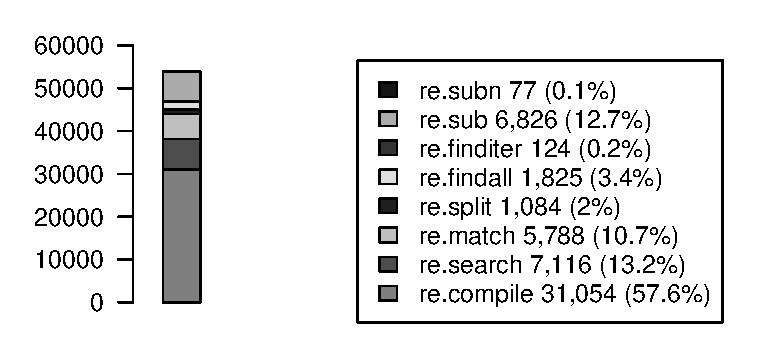
\includegraphics[width=\columnwidth]{nontex/illustrations/partFunctions.eps}
\vspace{-12pt}
\caption{How often are  {\tt re} functions used?}
\vspace{-6pt}
\label{fig:partFunctions}
\end{figure}

\begin{figure}[tb]
\centering
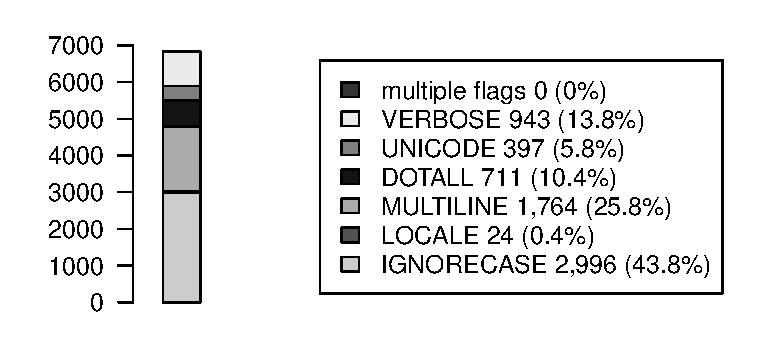
\includegraphics[width=0.9\columnwidth]{nontex/illustrations/partFlags.eps}
\vspace{-6pt}
\caption{Which behavioral flags are used?}
\vspace{-6pt}
\label{fig:partFlags}
\end{figure}


